\documentclass[11pt]{ctexart}


\usepackage[margin=2cm]{geometry}

\usepackage{graphicx}

\usepackage{listings}
\lstset{
	numbers=left,
	numberstyle=\tiny,
	basicstyle=\small,
	keywordstyle=\color{red},
	identifierstyle=,
	commentstyle=color{grey},
	stringstyle=\ttfamily,
	showstringspaces=false
}

\usepackage{url}

\title{\heiti{\LaTeX 总结}}
\author{\kaishu{北方以北}}
% \institute{国家知识产权局专利局专利审查协作河南中心}
\begin{document}

\maketitle

\tableofcontents

\section{序}

这是我关于自己在\LaTeX 学习和使用中笔记的整理和归纳,其中大部分来自于几年间在为知笔记中的收藏记录,少部分来自于其他人的一些课件或文章。这些内容都是零散的,我只是分门别类做了整理,因此如果想系统学习\LaTeX ,最好还是看官方的教程或书籍。

\section{\LaTeX 学习历程}

我从2010年开始接触到\LaTeX ,当时忘记了在哪个地方偶然看到了关于\LaTeX 的一些介绍文章,于是在自己的台式机上下载了\TeX Live,跟着指导一点一点学,但没有学习太深入。2011年上了研究生,我重新拾起了对\LaTeX 的兴趣,开始继续深入的学习,记得当时还去北邮的打印店把整本书都印了出来,并且在数值计算的结课上使用了一个期刊的\LaTeX 模板,老师还高高兴兴地给了我高分。现在想起来,大概是学数学的经常使用\LaTeX ,而其他专业的少人问津,当时的数学老师可能比较惊讶。我记得当时没有使用fontspec和XeCJK库,而是使用了MikTeX包和WinEdt编辑器。到了研究生二年级的时候,我接触了Beamer和XeCJK,并开始应用于幻灯片的制作。但是当时缺少系统和深入的学习,幻灯片制作得并不优雅美观。

我使用\LaTeX 最大的成就,就是用它完成了自己的硕士学位论文。在写学位论文时,我查找了大量的资料,后来使用了北邮一个毕业生的模板,做了稍许的修改。现在看来,\LaTeX 排出来的文章,确实在美观性上远好于Microsoft Word的效果。

工作以后的2014-2015年间,也断断续续地学了一些TikZ,也做了一些幻灯片,同时也全面转向了\CTeX 宏包。但是,由于做文档与单位的风格不同,做幻灯片也不够新颖美观,因此慢慢地少于使用。


我学习\LaTeX 完全出于兴趣,而非学习和工作的需要,并且由于以上断断续续的学习,目前我大概还处于初级使用者的水平,远谈不上深入,而且我预计以后的工作中,也会越来越少地使用\LaTeX ,但作为一项基本的书写技能,现在想把以前零碎的笔记做一个系统化的整理,以方便自己以后的使用,同时也希望有利于其他人的学习。

\section{\LaTeX 基本语法拾遗}
\LaTeX 是向后兼容的。

\subsection{排版基础}
在paper开头,必不可少的是会引用LaTeX packages。除了常用的\LaTeX 包,在此需要特别说明的有两个:一是\verb|\usepackage[american]{babel}|,另一个是\verb|\usepackage{microtype}|,引用这两个包会大大提升排版的正式程度和美观程度。其中\verb|\usepackage[american]{babel}|的引用是遇单词换行的时候,确保单词的切割是按照音节来而不是随意切割。这会让作为native speaker的审稿人赏心悦目,心中暗爽。而\verb|\usepackage{microtype}|的最大特点就是能够调整全篇文章(或局部)的字间距,字间距最大调整范围为±1em。可使得某段落不会出现单独一个单词占一行,或文章末尾单独一行文字占一页的不美观情况。\footnote{该包在NIPS中自带引用,而ECCV由于LNCS在排版方面的一些限制因素,不推荐在ECCV中使用该包引用}

在行文过程中若使用括号,括号前一定要有空格与前文内容分开。这也是中文作者很容易忽略的一点。例如,“the boosting algorithm (AdaBoost)” “the clustering algorithm (k-means)”。

单双引号的使用。正确的单引号使用方式:左引号为 (全键盘上数字1左侧键位),右引号为 ' (分号右侧键位)。双引号则重复输入两次即可(即 '')。切记不是平常引号的输入方式。

脚注使用时如遇句尾,则应该在句尾标点符号后引用,具体为:“respectively.\verb|\footnote{blablabla}”|。这样是为了防止句尾是数字的情形产生误读:如果是数字,footnote的标号就很可能被误认为数字的次方。

一些英文简写的用法。“that is”写作“i.e.,”,“for example”写为“e.g.,”,而“参看/参考”简写为“cf.”。注意,前两者有两个“.”且末尾要有“,”而“参考”的简写只有一个“.”。

文中在引用参考文献时要用“\~{}”(而不是直接空格)来产生空格。例如,“state-of-the-art MIL algorithms, e.g., miFV\~{}\verb|\cite{bibmiFV}| and miGraph\~{}\verb|\cite{bibmiGraph}|, and …” 用“\~{}”来产生空格的好处是使得“miFV [5]”作为一个整体,在换行时不会发生“[5]”与前文分开而单独处于行首的错误情况。“\~{}\verb|\ref{}|”命令同理。

为产生目录中的简写形式,可使用\verb|\caption[short text]{long text}|,其中方括号中为简写形式。

段落结尾时,不要使用\verb|\\|,使用双反斜杠是为了本段继续书写。

如果编译时出错,可在出错前的命令前添加\verb|\protect|用于调试,但应修复错误。

\LaTeX 类及宏包是在\verb|\leftmark|和\verb|\rightmark|中存储章节编号的。

为改变输出尺寸,可使用\verb|landscape|宏包。页面布局可使用宏包\verb|typearea|。页面间距可使用\verb|geometry|宏包。

\LaTeX 默认行间距为行高的20\% ,为调整行间距,可使用\verb|setspace|宏包,其具有选项\verb|onehalfspacing|可将行间距调整为1.5倍行高。宏包\verb|parskip|可用于取消\emph{段落}的缩进,此宏包中还包括段落间的距离调整功能。

英文中常用到连笔,但有些PDF阅读软件并不支持连笔的搜索和复制,此时可在\verb|microtype|宏包中设置\verb|noligatures|选项来进行取消。

命令\verb|\xspace|可根据不同的情形添加空格:后面跟一个单词时,加入一个空格;如果后面是英文的句号、逗号、叹号和引号则不添加空格。

\subsection{页眉页脚}
普通的页眉页脚可以使用\verb|\pagestyle{plain}|或\verb|\pagestyle{headings}|,前者不产生页眉页脚,后者产生普通的页眉页脚。

为产生更丰富形式的页眉页脚,可使用fancyhdr宏包来定制,引入宏包后使用\verb|\pagestyle{fancy}|来定制具体的格式。

\subsection{字体}
使用命令\verb|\sffamily|可将当前字符的字体切换为无衬线字体。

\subsection{数学公式排版}
文中,特别是在equation环境下,如果要插入公式,则公式后一定要有标点“逗号”或“句号”。使用方法:在公式后加入“\verb|\,,|”(逗号)或“\verb|\,.|”(句号)即可。不推荐使用\verb|\text{,}|或\verb|\text{.}|。因为\verb|\text{}|环境下的标点长相与“\verb|\,,|”或“\verb|\,.|”不同,且“\verb|\,,|”或“\verb|\,.|”前会自动与公式隔出一段距离,更加正式、美观。

公式中的\verb|\ldots|和\verb|\cdots|。“\verb|\ldots|”是列举中的省略符号,而“\verb|\cdots|”用于运算(如连加、连乘等)中的省略,二者主要区别在于位置一高一低,切勿混用。

公式中如果有指数或对数表示,要用\verb|\exp|或\verb|\log|命令。不能用\verb|\text{exp}|或\verb|\text{log}|,更不能直接输入exp或log来表示。

在很多机器学习和视觉文章中会用到范数,正确的一范数或二范数表示应为\verb|$\ell_1$或$\ell_2$|,输出为$\ell_1$或$\ell_2$。

公式中的单位向量或零向量要用向量写法:\verb|\vec{1}| 或\verb|\vec{0}|,有时也用\verb|\bm{1}|加粗来表示向量,否则会被误认为标量。

\verb|\left \right|:可以用.匹配不存在的左右部分 

矩阵分块:在array环境中加线,类似tabular, 

虚线:用arydshln宏包 

用\verb|;{}|代替竖线条 

用\verb|\hdashline|代替代替\verb|\hline|,或下载pmat宏包

图\ref{fig:greeks}是希腊字母的命令表示。
\begin{figure}[htpb]
\centering
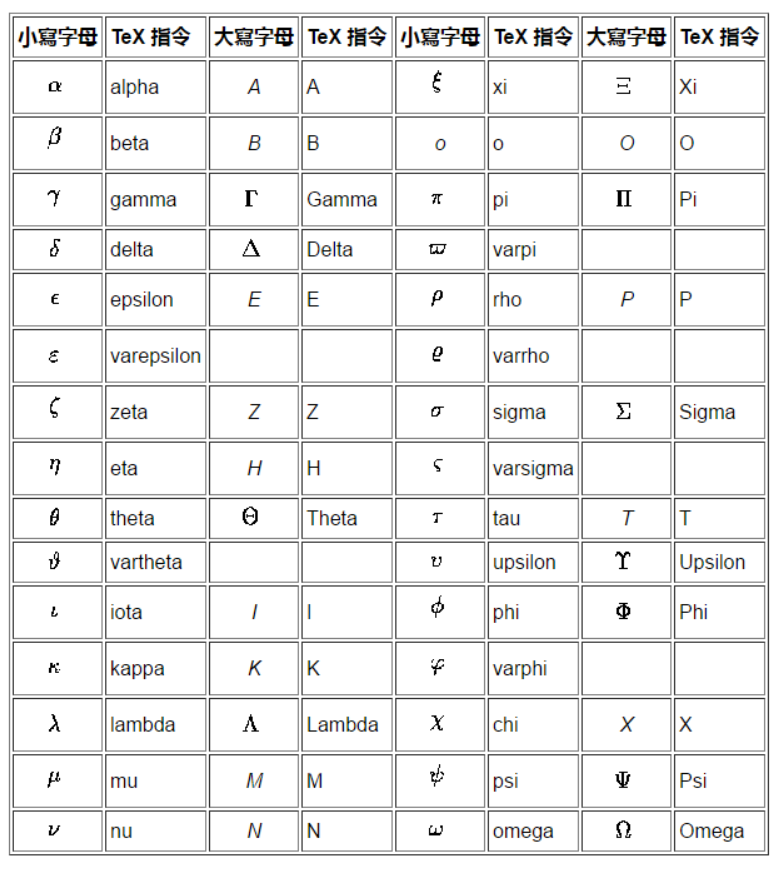
\includegraphics[width=0.7\linewidth]{greeks.png}
\caption{希腊字母的命令表示。}\label{fig:greeks}
\end{figure}


\subsection{表格排版}
表格的多列示例:
\begin{verbatim}
\multirow{number of rows}{width}{entry text}
\multicolumn{number of columns}{formatting options}{entry text}
\end{verbatim}

\subsubsection{彩色表格}
使用\verb|colortbl|宏包可制作彩色表格,主要使用的命令是\verb|\columncolor|和\verb|rowcolor|,前者给列进行着色,后者给行进行着色。代码如下\footnote{参见\url{http://tex.stackexchange.com/questions/176220/fancy-colored-array-in-latex}}:
\begin{lstlisting}[language=tex]
\documentclass[a4paper,12pt]{article}
\usepackage[left=1.5cm,right=1.5cm,top=1.5cm,bottom=1.5cm,ignoreheadfoot]{geometry}
\usepackage{array}
\usepackage[svgnames,table]{xcolor}
 
\newcommand*{\arraycolor}[1]{\protect\leavevmode\color{#1}}
\newcolumntype{A}{>{\columncolor{blue!50!white}}c}
\newcolumntype{B}{>{\columncolor{LightGoldenrod}}c}
\newcolumntype{C}{>{\columncolor{FireBrick!50}}c}
\newcolumntype{D}{>{\columncolor{Gray!42}}c}
 
\begin{document}    
 
\begin{center}
\sffamily
\arrayrulecolor{white}
\arrayrulewidth=1pt
\renewcommand{\arraystretch}{1.5}
\rowcolors[\hline]{3}{.!50!White}{}
\begin{tabular}{A|B|C}
  \multicolumn{3}{D}{\bfseries Example table}\\
  \rowcolor{.!50!Black}
  \arraycolor{White}\bfseries First column &
  \arraycolor{White}\bfseries Second column&
  \arraycolor{White}\bfseries Third column\\
  1 & A & E\\
  2 & B & F\\
  3 & C & G\\
  4 & D & H\\
\end{tabular}
\end{center}
 
\end{document}
\end{lstlisting}

得到的表格图\ref{fig:colortbl}所示。
\begin{figure}[htpb]
\centering
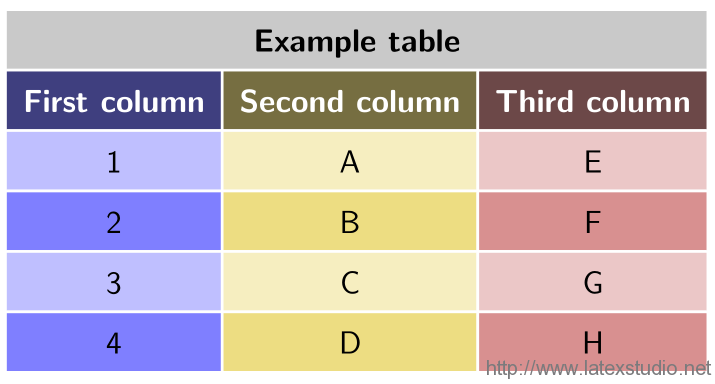
\includegraphics[width=0.5\linewidth]{colortbl.png}
\caption{彩色表格示例。}\label{fig:colortbl}
\end{figure}


\subsection{插图排版}
若文章需要插入很多图片,那么直接和\verb|“.tex”|放在一起就会很杂乱。这时可在\verb|”.tex”|所在目录下新建名为“figure”的文件夹,将图片放入figure文件夹后调用\verb|\graphicspath{{figure/}}|命令即可。

可将\verb|\vspace{-1em}|放置于figure或table的\verb|\caption|和图片或表格主体之间,来缩小空白节省篇幅。当然,如果会议或期刊明确要求了图片主体与图片标题的间距,则不要使用该命令!

插入图片时需要估算本页还有多少空间可用,下面的示例可以根据这个空间来确定图片的高度:
\begin{verbatim}
\includegraphics[
  height=\dimexpr\pagegoal-\pagetotal\relax,
  width=\textwidth,
  keepaspectratio]{graph} 
\end{verbatim}

\subsection{参考文献}
若某文献标题中含有特定含义大写字母(“SVM” “EM”等),应特别用第二重\verb|{}|将其括起来才可使其正常表示。如,“Title = \verb|{{EM-DD}|: An improved multiple-instance learning technique\verb|}|”。

\subsection{插入代码}
可以直接使用\verb|\verb||code|来使用latex中的代码,或通过verbatim环境。

\section{\LaTeX 中文排版}

\section{Beamer拾遗}

\subsection{插入代码}
在Beamer中插入代码,应当在frame环境中加入\verb|[fragile]|选项再使用verbatim宏包。

\section{文档类编写}

\section{总结}

\end{document}